\documentclass[12pt]{article}
\usepackage{float}
\usepackage[dvipsnames]{xcolor}
\usepackage{dingbat, tikz}
\usepackage{amsfonts,amsmath, color, fullpage, graphicx, mathtools, empheq, amsthm, amssymb}
\usepackage{wasysym}
\usepackage{thmtools}
\usepackage{listings}
\usepackage[framed]{mcode}

\newtheorem{problem}{Problem}

%To allow for matrix larger than 10x10
\setcounter{MaxMatrixCols}{11}

%To set thumbs up as QED symbol
\renewcommand{\qedsymbol}{\begingroup \color{blue} \rightthumbsup \endgroup}

%To make a new command for an asterisk in a circle
\newcommand{\circlesign}[1]{ 
    \mathbin{
        \mathchoice
        {\buildcirclesign{\displaystyle}{#1}}
        {\buildcirclesign{\textstyle}{#1}}
        {\buildcirclesign{\scriptstyle}{#1}}
        {\buildcirclesign{\scriptscriptstyle}{#1}}
    } 
}
\newcommand\buildcirclesign[2]{%
    \begin{tikzpicture}[baseline=(X.base), inner sep=0, outer sep=0]
    \node[draw,circle] (X)  {\ensuremath{#1 #2}};
    \end{tikzpicture}%
}

%To use a border matrix with brackets
\usepackage{etoolbox}
\let\bbordermatrix\bordermatrix
\patchcmd{\bbordermatrix}{8.75}{4.75}{}{}
\patchcmd{\bbordermatrix}{\left(}{\left[}{}{}
\patchcmd{\bbordermatrix}{\right)}{\right]}{}{}



\def\C{\mathbb{C}}
\def\N{\mathbb{N}}
\def\Q{\mathbb{Q}}
\def\R{\mathbb{R}}
\def\Ts{\mathbb{T}}
\def\Z{\mathbb{Z}}
\def\T{\mathcal{T}}
\def\P{\mathcal{P}}
\title{\underline{Math 226B: Homework \#3}}
\author{\huge Kara Gorman}
\begin{document}
\maketitle


\bigskip\bigskip
\noindent
\begin{problem} Consider the two-dimensional Poisson's equation on the unit square,
$$-\frac{\partial^2 v(x,y)}{\partial x^2} - \frac{\partial^2 v(x,y)}{\partial y^2} = f(x,y), \text{ } 0<x,y<1,$$
together with boundary conditions of the form
\begin{align}
v(x,0) &= b_0(x), \text{ } 0<x<1 \nonumber \\
v(x,1) &= b_1(x), \text{ } 0<x<1, \nonumber \\
v(0,y) &= c_0(y), \text{ } 0<y<1, \nonumber \\
v(1,y) &= c_1(y), \text{ } 0<y<1. \nonumber 
\end{align}
\end{problem}

\begin{itemize}
\item[(a)] Generalize the fast FFT-based solver for zero boundary conditions, which was presented in class, to general boundary conditions.\\

To generalize the FFT-based solver we did in class for general boundary conditions, let $m$ be the number of grid points.  Then, the distance between each grid point is $h := frac{1}{m+1}$.  Then, at the grid points, $(x_j, y_k) = (jh, kh)$.  So,  $V_{jk} = V(x_j,y_k)$ is an $m\times m$ matrix and we can rewrite the boundary conditions as: 
\begin{align}
v_{m+1,k} &= b_0, \text{ } k=1,\dots , m \nonumber \\
v_{0,k} &= b_1, \text{ } k=1, \dots , m \nonumber \\
v_{j,0} &= c_0, \text{ } j=1, \dots , m \nonumber \\
v_{j,m+1} &= c_1, \text{ } j=1, \dots , m \nonumber 
\end{align}

Now, we can write the centered-difference approximation as follows:
$$4v_{jk} - v_{j-1,k} - v_{j+1,k} - v_{j,k-1} - v_{j,k+1} = h^2f_{jk} \text{ , } j,k = 1, \dots , m,$$
where $f_{jk} = f(x_j,y_k)$ for $j,k = 1, \dots , m$.\\

Now, we can see that the boundary conditions come in when $j = 1,m$ and $k=1,m$.  As seen in the centered-difference approximation equations, when $j=1$, then $v_{j-1,k} = v_{0,k} = b_1$ for $k=1, \dots,m$.  Similarly, when $j=m$, $v_{j+1,k} = v_{m+1,k} = b_0$ for $k=1, \dots,m$.  When $k=1$, $v_{j,k-1} = v_{j,0} = c_0$ for $j=1, \dots,m$.  And, when $k=m$, $v_{j,k+1} = v_{j,m+1} = c_1$ for $j=1, \dots,m$.  So, we need to account for this in our $m\times m$ matrix f by adjusting the first and last row and column as follows:
\begin{align}
f(1,:) &= f(1,:) + \frac{b_0}{h^2} \nonumber \\
f(m,:) &= f(m,:) + \frac{b_1}{h^2} \nonumber \\
f(:,1) &= f(:,1) + \frac{c_0}{h^2} \nonumber \\
f(:,m) &= f(:,m) + \frac{c_0}{h^2} \nonumber 
\end{align}
where $b_0, b_1, c_0, c_1$ are all vectors of length $m$.\\

Then, we proceed exactly as we did in class for the case of zero boundary conditions, execpt we use the $f$ defined above with out general boundary conditions.\qed\\\\



\item[(b)] Write a Matlab program that implements your FFT-based solver from (a) using Matlab's "fft".\\

\lstset{language=matlab,frame=single}
\begin{lstlisting}[caption= FFT-Based Solver with Generalized BCs]
function V = fft2DPoisson(m,b0,b1,c0,c1,f)

format long e

h = 1/(m+1);

f(1,:) = f(1,:) + 1/(h^2)*b0;
f(m,:) = f(m,:) + 1/(h^2)*b1;
f(:,1) = f(:,1) + 1/(h^2)*c0';
f(:,m) = f(:,m) + 1/(h^2)*c1';

% compute f'=z^T*f*z
f = fftMult(f);
f = fftMult(f')';

[X,Y]=meshgrid(1:m,1:m);

lambda = 2*(1 - cos(pi*h.*X) + 1 - cos(pi*h.*Y));
V_bar = (h^2)*f./lambda;

% compute V=z*V'*z^T
V = fftMult(V_bar);
V = fftMult(V')';


% function to do matrix-vector multiplication using fft
    function w = fftMult(A)
        
        n = size(A,2);
        A_tilde = [zeros(1,n); A; zeros(n+1,n)];
        w_tilde = fft(A_tilde);
        w_hat = w_tilde(2:n+1,:);
        w = -sqrt(2*h)*imag(w_hat);
        
    end
end
\end{lstlisting}
\qed\\\\




\item[(c)]  To test your Matlab program, use test cases that have solutions of the form
$$v(x,y) = y^\alpha \sin(\beta\pi x)\cos(\gamma\pi y),$$
where $\alpha \geq 0$ and $\beta,\gamma > 0$ are parameters.  Determine the functions $f$, $b_0$, $b_1$, $c_0$, and $c_1$ so that the function is indeed the solution of the above Poisson's equation.\\

To find $b_0$, $b_1$, $c_0$, and $c_1$, we simply plug in the boundary conditions defined in the problem statement into the given solution equation $v(x,y)$, as follows:
\[\begin{cases}
v(x,0) = 0^\alpha\sin(\beta\pi x) = b_0 \nonumber \\
v(x,1) = \sin(\beta\pi x)\cos(\gamma\pi) = b_1 \nonumber \\
v(0,y) = 0 = c_0 \nonumber \\
v(1,y) = y^\alpha\sin(\beta\pi)\cos(\gamma\pi y) = c_1 \nonumber 
\end{cases}\]

Now, we can find $f$ by staking the sum of the second partial derivatives of $v(x,y)$ as follows:
\begin{align}
\frac{\partial v}{\partial x^2} &= -\beta^2\pi^2y^\alpha\sin(\beta\pi x)\cos(\gamma\pi y) \nonumber \\
\frac{\partial v}{\partial y^2} &= (-\pi^2\gamma^2y^\alpha y^\alpha + (\alpha - 1)\alpha y^{\alpha - 2})\sin(\beta\pi x)\cos(\gamma\pi y) - 2\pi\alpha\gamma y^{\alpha - 1}\sin(\gamma\pi y)\sin(\beta\pi x) \nonumber
\end{align}

Then,
\begin{align}
f &= -\frac{\partial v}{\partial x^2} - \frac{\partial v}{\partial y^2} \nonumber \\
&= ((-\pi^2\gamma^2y^\alpha - \beta^2\pi^2 )y^\alpha + (\alpha - 1)\alpha y^{\alpha - 2})\sin(\beta\pi x)\cos(\gamma\pi y) - 2\pi\alpha\gamma y^{\alpha - 1}\sin(\gamma\pi y)\sin(\beta\pi x) \nonumber
\end{align}


\lstset{language=matlab,frame=single}
\begin{lstlisting}[caption= Function To Approximate \text{$V(x,y)$} with Given BCs]
function [abs_error] = fft2DPoissonSolver(m,alpha,beta,gamma)

format long e

h = 1/(m+1);

x = [h:h:1-h];
y = [h:h:1-h];

[X,Y] = meshgrid(x,y);

% construct f matrix
f = (beta^2)*(pi^2).*(Y.^alpha).*sin(beta*pi.*X).*cos(gamma*pi.*Y)...
  + (pi^2)*(gamma^2).*(Y.^alpha).*sin(beta*pi.*X).*cos(gamma*pi.*Y)...
  + 2*pi*alpha*gamma.*(Y.^(alpha-1)).*sin(gamma*pi.*Y).*sin(beta*pi.*X)...
  - (alpha - 1)*alpha.*(Y.^(alpha - 2)).*cos(gamma*pi.*Y).*sin(beta*pi.*X);
        

% construct boundary conditions vectors
    if alpha == 0
        b0 = sin(beta*pi.*x);
    else
        b0 = zeros(1,m);
    end

b1 = sin(beta*pi.*x).*cos(gamma*pi);
c0 = zeros(1,m);
c1 = sin(beta*pi).*(y.^alpha).*cos((gamma*pi).*y);

% call Poisson solver with boundary conditions, and f as inputs
V = fft2DPoisson(m,b0,b1,c0,c1,f);

% construct exact solution matrix v_exact
v_exact = (Y.^alpha).*sin((beta*pi).*X).*cos((gamma*pi).*Y);

% compute absolute error
[max_V, max_ind] = max(V(:));
[row_ind, col_ind] = ind2sub(size(V),max_ind);
abs_error = abs(max_V - v_exact(row_ind,col_ind))


hold on

subplot(1,3,1)
mesh(X,Y,f);
xlabel('x'); ylabel('y'); zlabel('f');
title('f(x,y)');


subplot(1,3,2);
mesh(X,Y,V);
xlabel('x'); ylabel('y'); zlabel('V');
title('Approximate solution of V(x,y)')

subplot(1,3,3)
mesh(X,Y,v_exact);
xlabel('x'); ylabel('y'); zlabel('v_exact');
title('Exact V(x,y)');

end
\end{lstlisting}
\qed\\\\


\item[(d)]  Use your FFT-based solver to compute approximate values
$$v_{jk} \approx v(x_j, y_k)$$
for the exact solution at the grid points $(x_j,y_k)$.  For each of your runs, determine the absolute error
$$\max_{j,k=1,2,\dots,m}|v_{jk} - v(x_j,y_K)|$$
of your computed solution.  Choose $m$ large enough so that the absolute error is below $5\times 10^{-4}$ and print out the $m$ you have used, together with the corresponding value of the absolute error.\\
Use the following 5 test cases:
\begin{itemize}
\item[(i)] $\alpha = 0$, $\beta = 1$, $\gamma = 0.5$;

\item[(ii)] $\alpha = 1$, $\beta = 1.5$, $\gamma = 2$;

\item[(iii)] $\alpha = 2$, $\beta = 3$, $\gamma = 0.5$;

\item[(iv)] $\alpha = 5$, $\beta = 3$, $\gamma = 1$;

\item[(v)] $\alpha = 5$, $\beta = 5$, $\gamma = 3$;

\begin{table}[H]
\centering
\renewcommand{\arraystretch}{1.3}
%\begin{small}
\begin{tabular}{| c || c | c |}
\hline
Case & m & Absolute Error\\
\hline 
(i) &  30 &  6.933594287494849e-05 \\
(ii) &  20 & 1.220314020542457e-04  \\
(iii) &  60 &  3.765313287558691e-04 \\
(iv) & 50  &  2.391712195491946e-04 \\
(v) & 70  & 3.799707430462984e-04  \\
\hline
\end{tabular}
%\end{small}
\caption{m values and absolute error for FFT-based Poisson solver}
\end{table} 

\begin{figure}[H]
\center
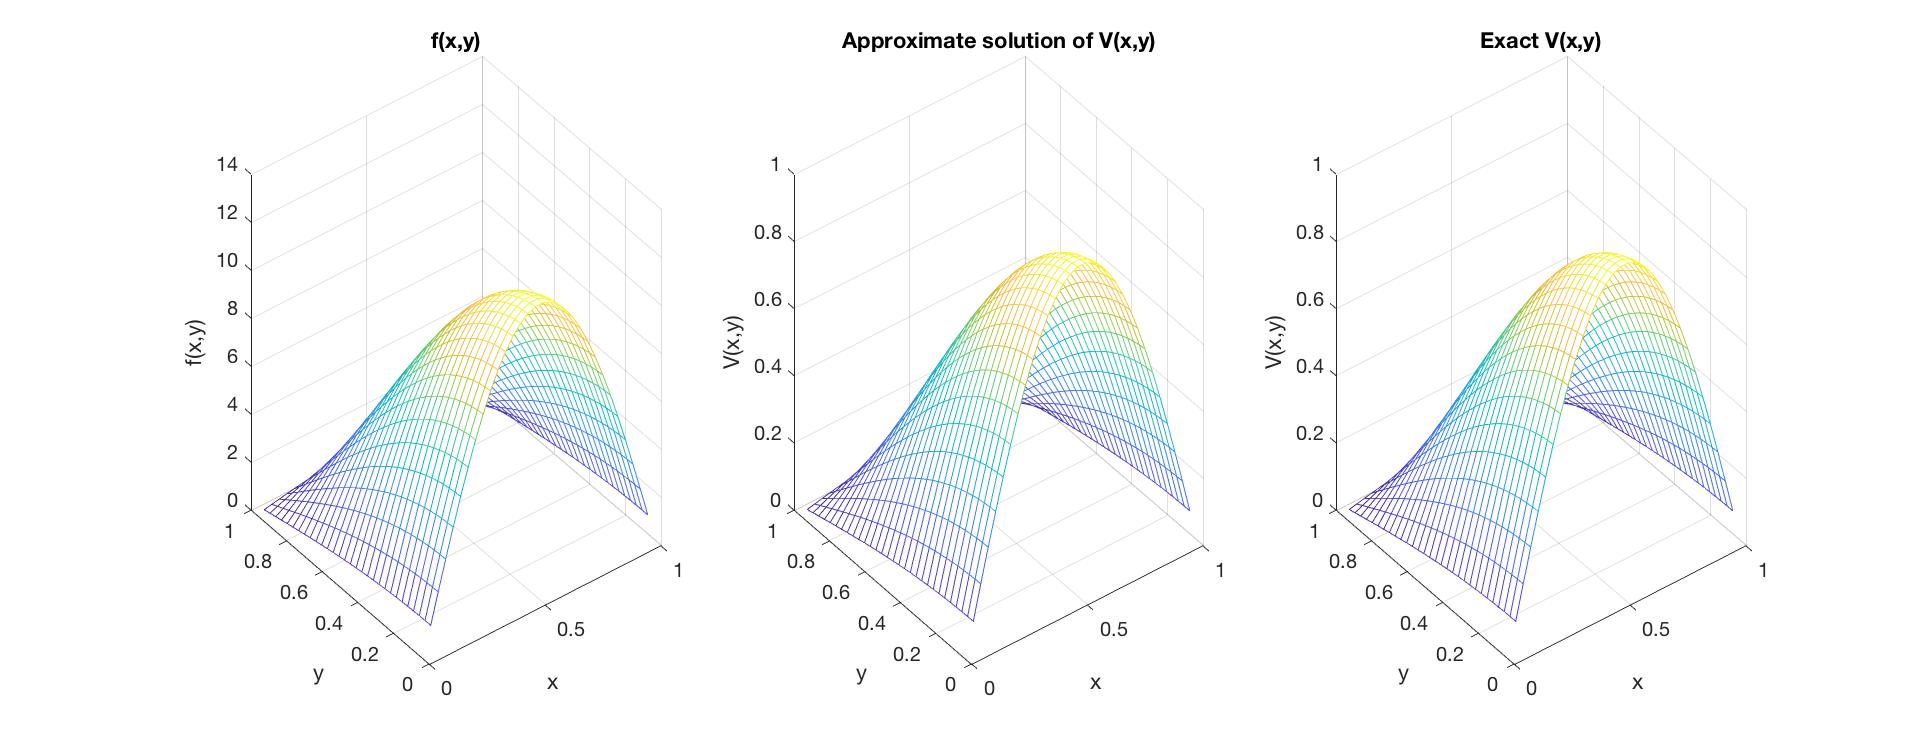
\includegraphics[scale=.25]{prob1casei.jpg}
\caption{3D Plots for Case (i)}
\end{figure}

\begin{figure}[H]
\center
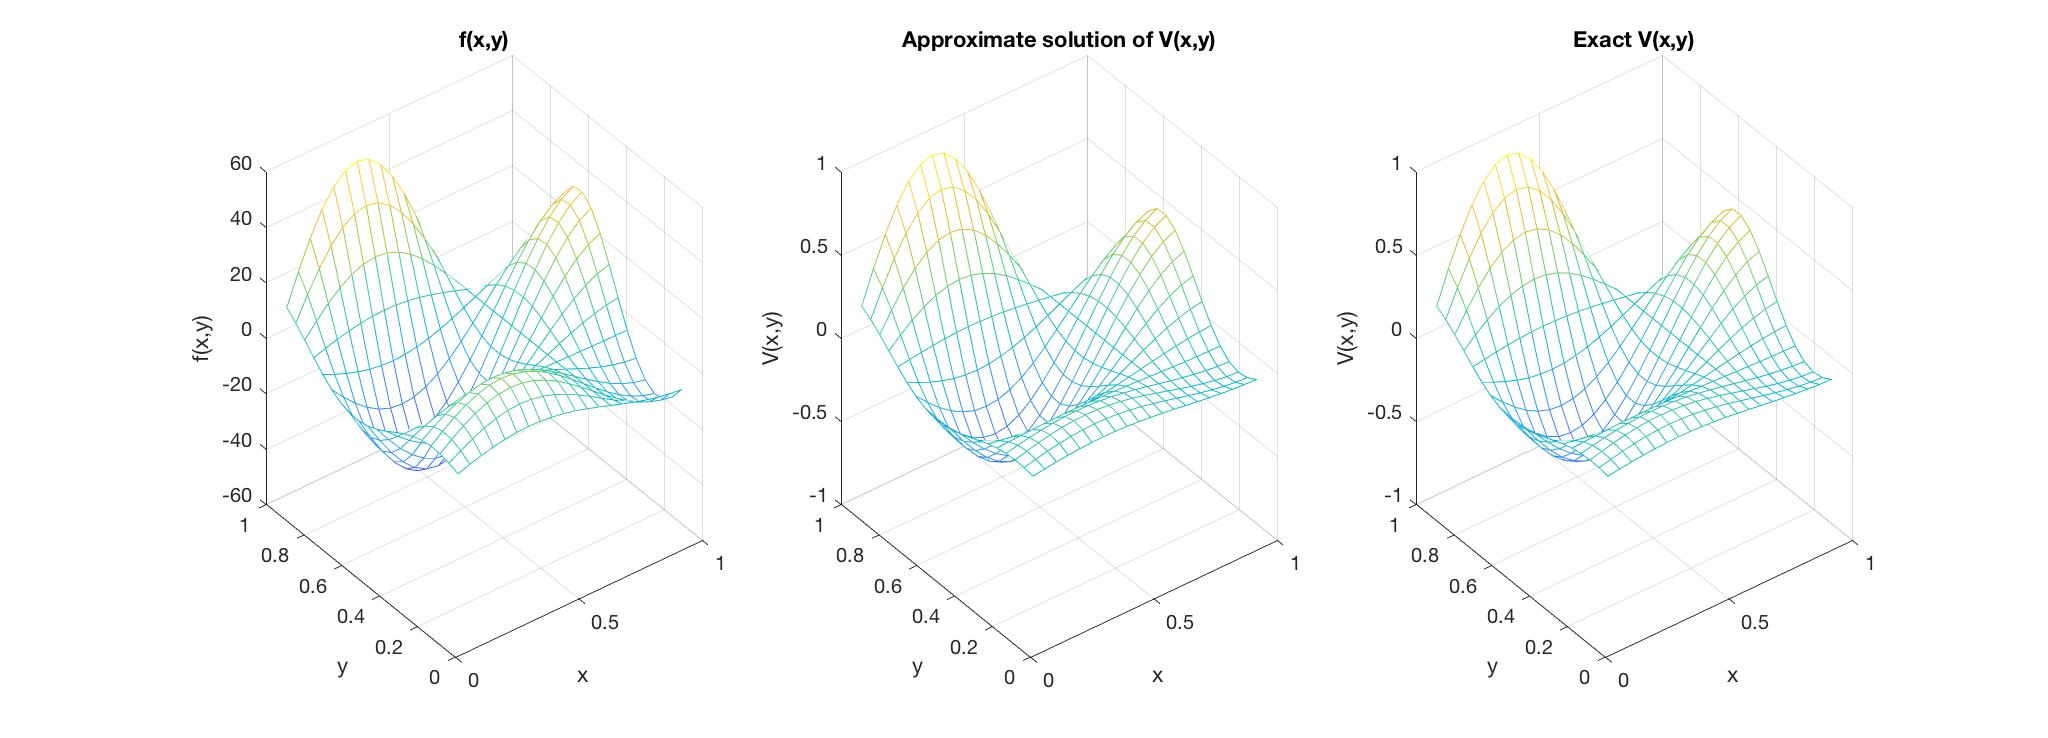
\includegraphics[scale=.25]{prob1caseii.jpg}
\caption{3D Plots for Case (ii)}
\end{figure}

\begin{figure}[H]
\center
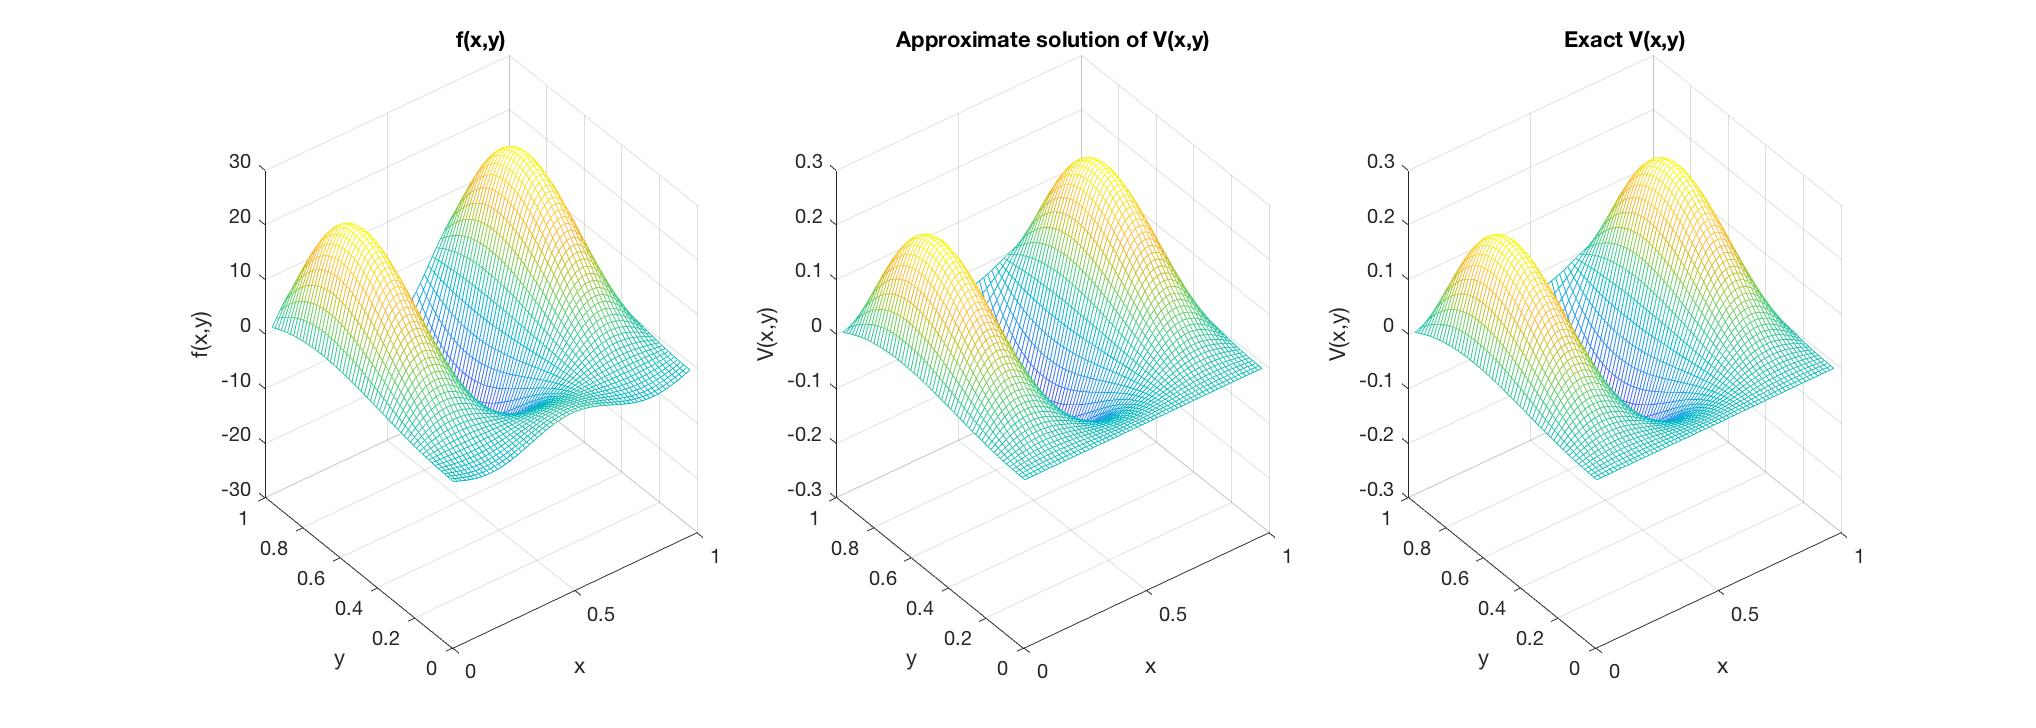
\includegraphics[scale=.25]{prob1caseiii.jpg}
\caption{3D Plots for Case (iii)}
\end{figure}

\begin{figure}[H]
\center
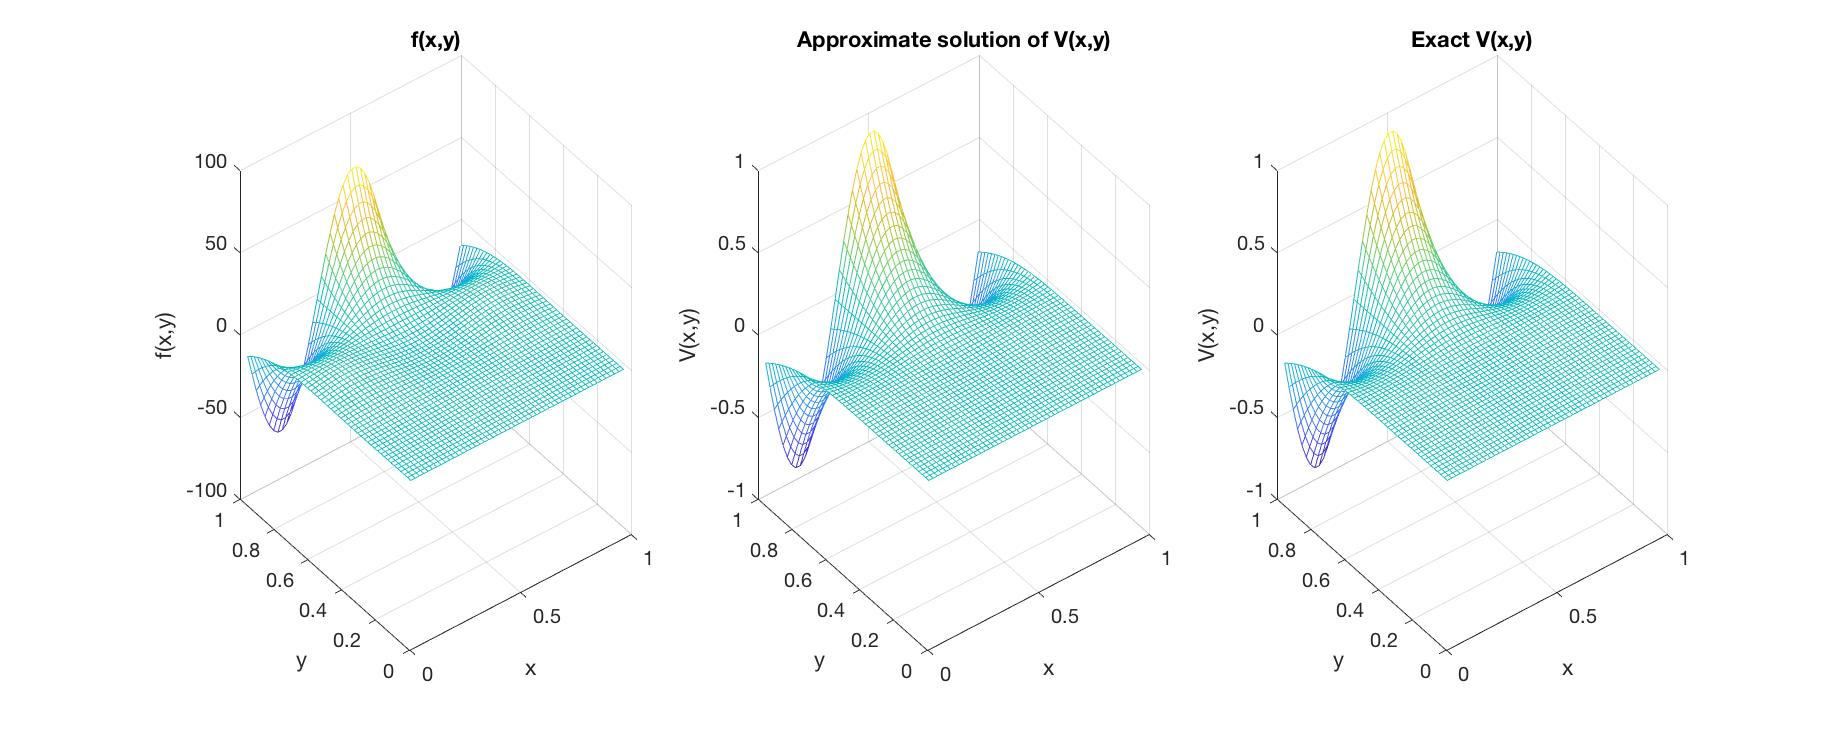
\includegraphics[scale=.28]{prob1caseiv.jpg}
\caption{3D Plots for Case (iv)}
\end{figure}

\begin{figure}[H]
\center
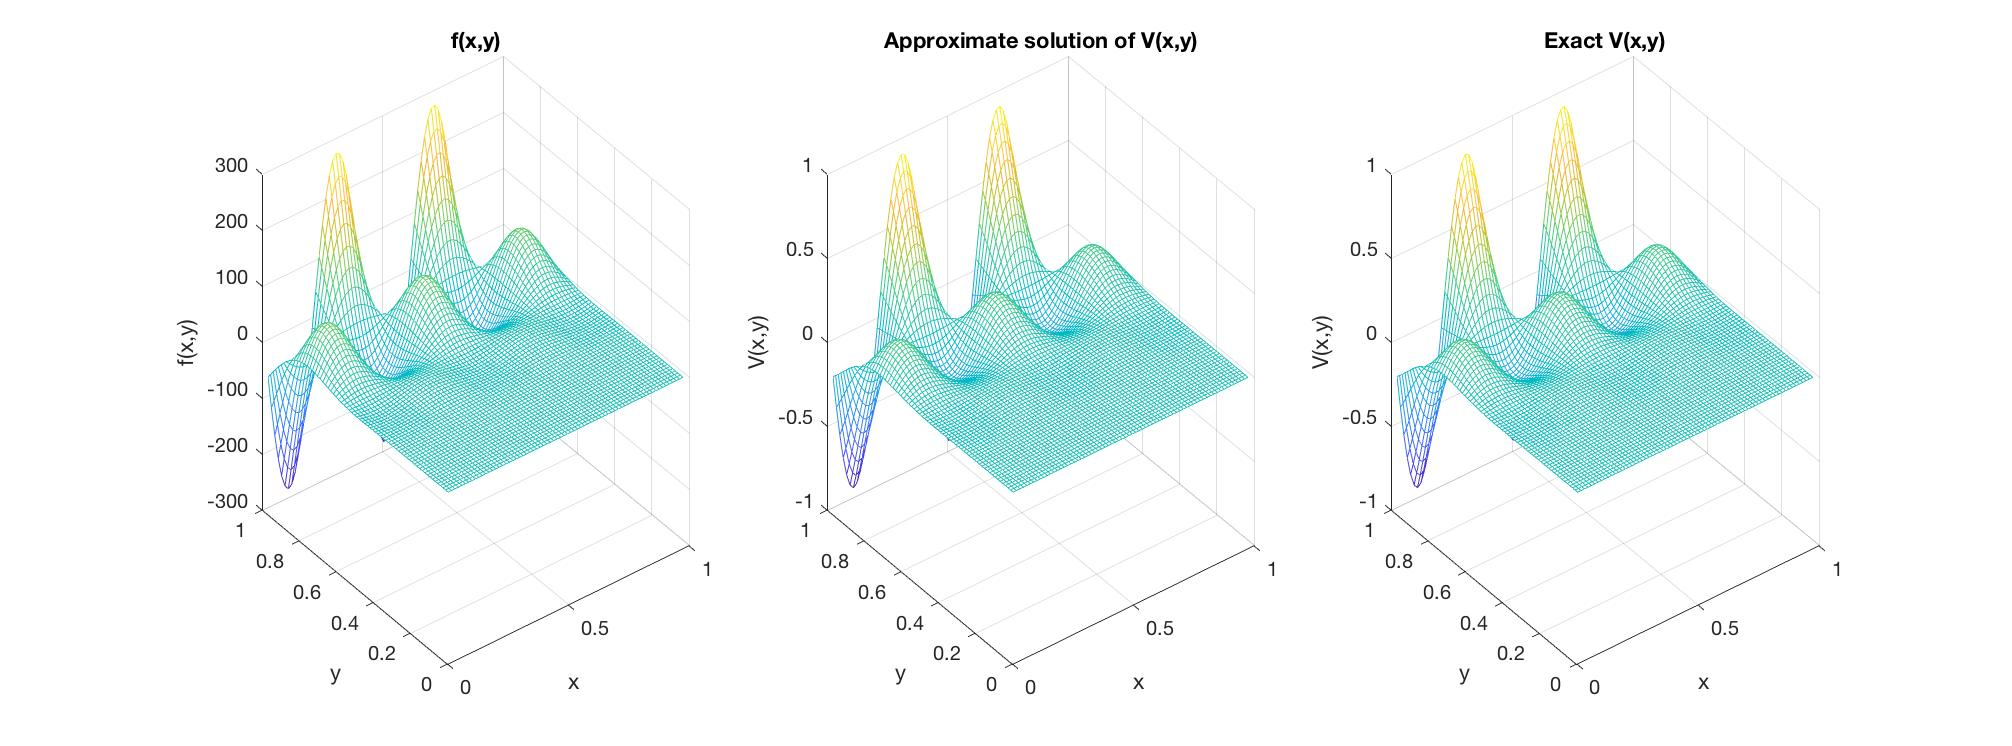
\includegraphics[scale=.25]{prob1casev.jpg}
\caption{3D Plots for Case (v)}
\end{figure}
\qed\\

\end{itemize}
\end{itemize}

\bigskip\bigskip
\noindent
\begin{problem} Consider two-dimensional partial differential equations of the following form:
$$-\frac{\partial^2 v(x,y)}{\partial x^2} - \frac{\partial^2 v(x,y)}{\partial y^2} +\sigma v(x,y) = f(x,y), \text{ } (x,y) \in R := (0,a)\times (0,b),$$
$$u = g(x,y), \text{ } (x,y) \in \partial R.$$
Here, $a, b, \sigma \in \R$ are constants with $a, b > 0$ and $\sigma \geq 0$, $f$ is a given function on $R$, and $g$ is a given function on $\partial R$.\\
The purpose of this problem is to generalize the solver presented in class to problems of the form above.  To this end, we discretize using grid points
$$(x_j,y_k) := (jh_x,kh_y), \text{ } j=0,1,\dots,m_x+1, \text{ } k=0,1,\dots,m_y+1,$$
where $m_x, m_y \geq 1$ are integers and
$$h_x := \frac{a}{m_x + 1} \text{ and } h_y := \frac{b}{m_y + 1}.$$
The usual centered differences are employed to approximate $\frac{\partial^2v(x,y)}{\partial x^2}$ and $\frac{\partial^2 v(x,y)}{\partial y^2}$.
\end{problem}

\begin{itemize}

\item[(a)] Show that the resulting discretization can be written in the form
$$T_{m_x}V + \alpha VT_{m_y} + \beta V = \tilde{F},$$
where the entries $v_{jk}$ of the matrix $V \in \R^{m_x \times m_y}$ are approximations to the solution $v(x,y)$ of the above Poisson equation at the interior grid points:
$$v_{jk} \approx u(x_j,y_k), \text{ } j=1,2,\dots,m_x, \text{ } k=1,2,\dots,m_y.$$

First, we need to compute the centered-difference approximations of $\frac{\partial^2v(x,y)}{\partial x^2}$ and $\frac{\partial^2 v(x,y)}{\partial y^2}$ as follows:
\begin{align}
-\frac{\partial^2v(x,y)}{\partial x^2} &\approx \frac{2v_{jk} - v_{j-1,k} - v_{j+1,k}}{h_x^2} \nonumber \\
-\frac{\partial^2 v(x,y)}{\partial y^2} &\approx \frac{2v_{jk} - v_{j,k-1} - v_{j,k+1}}{h_y^2} \nonumber 
\end{align}

So then our equation becomes:
\begin{align}
\frac{2v_{jk} - v_{j-1,k} - v_{j+1,k}}{h_x^2} + \frac{2v_{jk} - v_{j,k-1} - v_{j,k+1}}{h_y^2} +\sigma v_{jk} &= f_{jk} \nonumber \\
\frac{T_{m_x}V}{h_x^2} + \frac{VT_{m_y}}{h_y^2} + \sigma V &= F \nonumber 
\end{align}
where $T_{m_x} \in \R^{m_x \times m_x}$ and $T_{m_y} \in \R^{m_y \times m_y}$.\\

Now, multiplying both sides by $h_x^2$, we get:
\begin{align}
\frac{T_{m_x}V}{h_x^2} + \frac{VT_{m_y}}{h_y^2} + \sigma V &= F \nonumber \\
T_{m_x}V + \frac{h_x^2}{h_y^2}VT_{m_y} + h_x^2\sigma V &= h_x^2 F \nonumber \\
T_{m_x}V + \alpha VT_{m_y} + \beta V &= \tilde{F} \text{ \checkmark}\nonumber
\end{align}
Where $\alpha = \frac{h_x^2}{h_y^2}$, $\beta = h_x^2\sigma$, and $\tilde{F} = h_x^2F$.\qed\\\\


\item[(b)] Generalize the FFT-based algorithm presented in class so that you can use it to efficiently solve the equation in part (a).  How does the number of flops of your algorithm depend on $m_x$ and $m_y$?\\

First, we need to take into account the general boundary conditions.  From part (a), we have that the centered- difference approximation is:
$$\frac{2v_{jk} - v_{j-1,k} - v_{j+1,k}}{h_x^2} + \frac{2v_{jk} - v_{j,k-1} - v_{j,k+1}}{h_y^2} +\sigma v_{jk} = f_{jk}.$$

Then, as in Problem 1, we can see that the boundary conditions come in when $j=1$, $j=m_x + 1$, $k=1$, and $k=m_y + 1$.  When can see that when $j=1$, $v_{j-1,k} = v_{o,k} =: a_1$.  Similarly, when $j=m_x + 1$, $v_{j+1,k} = v_{m_x +2,k} =: a_0$.  When $k=1$, $v_{j,k-1} = v_{j,0} =: d_0$.  And, when $k=m_y + 1$, $v_{j,k+1} = v_{j,m_y + 2} =: d_1$.\\
So, our boundary conditions are:
\[\begin{cases}
g(x,0) = a_0(x) \\
g(x,b) = a_1(x) \\
g(0,y) = d_0(y) \\
g(a,y) = d_1(y) \\
\end{cases}\]
where $a_0(x), a_1(x) \in \R^{m_x}$ and $d_0(y), d_1(y) \in \R^{m_y}$.  We account for these general boundary conditions in $\tilde{F}$ by:
\[\begin{cases}
\tilde{F}(1,:) = \tilde{F}(1,:) + \frac{a_0}{h_x^2} \\
\tilde{F}(m_x + 1,:) = \tilde{F}(m_x + 1,:) + \frac{a_1}{h_x^2} \\
\tilde{F}(:,1) = \tilde{F}(:,1) + \frac{d_0}{h_y^2} \\
\tilde{F}(:,m_y + 1) = \tilde{F}(:,m_y + 1) + \frac{d_0}{h_y^2} \\
\end{cases}\]

No,w going back to the result of part (a), we see that:
\begin{align}
T_{m_x}V + \alpha VT_{m_y} + \beta V &= \tilde{F} \nonumber \\
\iff z^TT_{m_x}zz^TVz + \alpha z^TVzz^TT_{m_y}z + \beta z^TVz &= z^T\tilde{F}z \nonumber \\
\iff \Lambda_x V' + \alpha V'\Lambda_y + \beta V' &= \tilde{F}' \nonumber \\
\iff \lambda_{x_j}v'_{jk} + \alpha v'_{jk}\lambda_{y_k} + \beta v'_{jk} &= \tilde{f}'_{jk} \nonumber 
\end{align}
where $\Lambda_x := z^TT_{m_x}z$, $V' := z^TVz$, $\Lambda_y := z^TT_{m_y}z$, and $\tilde{F}' := z^T\tilde{F}z$.  Then, solving for $v'_{jk}$, we get:
\begin{align}
\lambda_{x_j}v'_{jk} + \alpha v'_{jk}\lambda_{y_k} + \beta v'_{jk} &= \tilde{f}'_{jk} \nonumber \\
\iff v'_{jk} = \frac{\tilde{f}'_{jk}}{\lambda_{x_j} + \alpha \lambda_{y_k} + \beta} \nonumber
\end{align}

So, we can generalize the algorithm presented in class as follows:\\

\underline{Algorithm:}\\
\begin{itemize}
\item Input: $m_x$, $m_y$, $F$, $\sigma$, $a$, $b$.
\item Output: The approximate solution to the 2D Poisson equation, $V \in \R^{m_x\times m_y}$.\\
\item Set $h_x := \frac{a}{m_x + 1}$; $h_y := \frac{b}{m_y + 1}$;
\item Set $\alpha := \frac{h_x^2}{h_y^2}$; $\beta := h_x^2\sigma$; $\tilde{F} := h_x^2F$;
\item Apply boundary conditions to $\tilde{F}$:\\
$\begin{cases}
\tilde{F}(1,:) = \tilde{F}(1,:) + \frac{a_0}{h_x^2} \\
\tilde{F}(m_x + 1,:) = \tilde{F}(m_x + 1,:) + \frac{a_1}{h_x^2} \\
\tilde{F}(:,1) = \tilde{F}(:,1) + \frac{d_0}{h_y^2} \\
\tilde{F}(:,m_y + 1) = \tilde{F}(:,m_y + 1) + \frac{d_0}{h_y^2} \\
\end{cases}$
\item (1) Compute $\tilde{F}' = z^T\tilde{F}z$.
\item (2) Set $v'_{jk} = \frac{\tilde{f}'_{jk}}{\lambda_{x_j} + \alpha \lambda_{y_k} + \beta}$.
\item (3) Compute $V' = z^TVz$.\\
\end{itemize}

\underline{Flop Count:}
\begin{itemize}
\item (1) 2 matrix-matrix multiplications:\\
$(2m_y - 1)m_ym_x + (2m_y - 1)m_xm_x = \begin{cases}
				\mathcal{O}(m_y^2m_x) & \text{ if } m_y \geq m_x \\
				\mathcal{O}(m_x^2m_y) & \text{ if } m_x > m_y. \\
										\end{cases}$
\item (2) $\mathcal{O}(m_xm_y)$.
\item (3) Same as (1):\\
$(2m_y - 1)m_ym_x + (2m_y - 1)m_xm_x = \begin{cases}
				\mathcal{O}(m_y^2m_x) & \text{ if } m_y \geq m_x \\
				\mathcal{O}(m_x^2m_y) & \text{ if } m_x > m_y. \\
										\end{cases}$
\end{itemize} 

So, the total flop count is: $\begin{cases}
				\mathcal{O}(m_y^2m_x) & \text{ if } m_y \geq m_x \\
				\mathcal{O}(m_x^2m_y) & \text{ if } m_x > m_y. \\
										\end{cases}$
\end{itemize}
\qed\\\\





\bigskip\bigskip
\noindent
\begin{problem}  Let $t_0, t_1, \dots , t_{n-1} \in R$ be given numbers such that the Toeplitz matrix
$$T = \left[t_{|k-j|}\right]_{j,k=1,2,\dots,n} \in \R^{n\times n}$$
is symmetric positive definite.  Let $\mathcal{C}_n$ denote the set of all circulant matrices $C \in \R^{n\times n}$.  Recall that
$$||A||_F = \left(\sum\limits_{j=1}^n\sum\limits_{k=1}^n a^2_{jk}\right)^{1/2}$$\\
\noindent
is the Frobenius norm of $A = \left[a_{jk}\right]_{j,k=1,2,\dots,n} \in \R^{n\times n}$.\\

\noindent
Determine a circulant matrix $C_T \in \mathcal{C}_n$ such that
$$||C_T - T||_F = \min\limits_{C \in \mathcal{C}_n} ||C - T||_F.$$
\noindent
Show that $C_T$ is unique.  Show that $C_T$ is symmetric.\\
\end{problem}

\begin{align}
||C_T - T||_F^2 &= \left(\sum\limits_{j=1}^n\sum\limits_{k=1}^n (c_{jk} - t_{|k-j|})\right) \nonumber \\
&= \left(trace((C_T - T)^T(C_T - T))\right) \nonumber \\
&= \left(trace((C_T^T - T^T)(C_T - T))\right) \nonumber \\
& = \left(trace(C^TC - C^TT - T^TC + T^TT)\right) \nonumber \\
& = \left(trace(C^TC - 2C^TT + T^TT)\right) \nonumber \\
&= \left(trace(C^TC) - 2*trace(C^TT) + trace(T^TT)\right) \nonumber
\end{align}

\noindent
Then, we find that:
\begin{align}
trace(C^TC) &= n\sum\limits_{i=1}^{n-1} c_i^2 
\end{align}

\begin{align}
trace(C^TT) &= \sum\limits_{k=1}^n\left(\sum\limits_{i=0}^{n-k} c_it_i + \sum\limits_{i=0}^k t_{-i}c_{k-1}\right) \nonumber \\
&= \sum\limits_{k=1}^n\sum\limits_{i=0}^{n-k} c_it_i + \sum\limits_{k=1}^n\sum\limits_{i=0}^{k} t_{-i}c_{k-1}
\end{align}
\noindent
Since we are going to be taking the derivatives of each term with respect to $C_i$, then we don't care what $trace(T^TT)$ is because it doesn't contain any $C_i$ terms, so the derivative will be zero.  So, taking the gradient of (1) and (2), we get:
\begin{align}
\nabla(trace(C^TC)) &= 2n\sum\limits_{i=1}^{n-1} c_i \nonumber \\
&= 2n\begin{bmatrix}
		c_0 \\
		c_1 \\
		c_2 \\
		\vdots \\
		c_{n-1} \\
	\end{bmatrix} \nonumber
\end{align}
\noindent
and,
\begin{align}
\nabla(trace(C^TT)) &= \begin{bmatrix}
						nt_0 \\
						(n-1)t_1 + t_{-(n-1)} \\
						(n-2)t_2 + 2t_{-(n-2)} \\
						\vdots \\
						t_{n-1} + (n-1)t_{-1} \\
						\end{bmatrix} \nonumber
\end{align}
\noindent
So, it follows that:
$$n\begin{bmatrix}
		c_0 \\
		c_1 \\
		c_2 \\
		\vdots \\
		c_{n-1} \\
	\end{bmatrix} = \begin{bmatrix}
						nt_0 \\
						(n-1)t_1 + t_{-(n-1)} \\
						(n-2)t_2 + 2t_{-(n-2)} \\
						\vdots \\
						t_{n-1} + (n-1)t_{-1} \\
						\end{bmatrix}.$$
\noindent						
Thus, a circulant matrix $C_T$ that satisfies the conditions is defined by:
\begin{align}
c_j &= \frac{1}{n}\left[(n-j)t_j + jt_{-(n-j)}\right] \nonumber \\
\Aboxed{c_j &= \frac{1}{n}\left[(n-j)t_j + jt_{(n-j)}\right]} \text{ for all $j=0,1,\dots, n-1$} \nonumber
\end{align}
where $t_{-(n-j)} = t_{(n-j)}$ since $T$ is symmetric, positive definite.\\

\noindent
By the way we constructed $C_T$, it is clear that it is unique.\\

\noindent
To show $C_T$ is symmetric, we want to show that $c_j = c_{n-j}$.
\begin{align}
c_{n-j} &= \frac{1}{n}\left[(n-n+j)t_{n-j} + (n-j)t_{(n-n+j)}\right] \nonumber \\
&= \frac{1}{n}\left[jt_{n-j} + (n-j)t_{j}\right] \nonumber \\
&= \frac{1}{n}\left[jt_{-(n-j)} + (n-j)t_j\right] \nonumber \\
&= \frac{1}{n}\left[(n-j)t_j + jt_{(n-j)}\right] \nonumber \\
&= c_j \text{ \checkmark} \nonumber
\end{align}

\noindent
Thus, $C_T$ is symmetric.\\
\qed


\newpage
\bigskip\bigskip
\noindent
\begin{problem}
\end{problem}

\begin{itemize}

\item[(a)]  Write a Matlab routine based on your algorithm from Problem 5(d) of Homework 1 and Matlab's "pcg" for solving linear systems $Tx = b$ by the means of the CG method.\\

\lstset{language=matlab,frame=single}
\begin{lstlisting}[caption= Function to Solve the Linear System \text{$Tx=b$,} for \text{$T$} Toeplitz]
function [x] = ToeplitzPCG(p,n)

format long e 

tol = 10^(-9);
maxit = n;

b = ones(n,1);

i=(1:n);
t = 1./((1 + sqrt(i-1)).^p);

[x,flag,relres,iter] = pcg(@TmultFunct,b,tol,maxit);

    % function to do matrix-vector multiplication using FFT
    function y = TmultFunct(z)
        y = fftToeplitz(t,z);
        
    end
end
\end{lstlisting}

\lstset{language=matlab,frame=single}
\begin{lstlisting}[caption=]
function [y] = fftToeplitz(t,x)

n = length(x);

c = zeros(1,2*n-1);
c(1:n) = t(1:n);
c(n+1:2*n-1) = t(n:-1:2);

x_tilde = zeros(2*n-1,1);
x_tilde(1:n) = x;

c = c';

y_tilde = fftCirculant(c,x_tilde);

y = y_tilde(1:n);
end
\end{lstlisting}

\newpage
\lstset{language=matlab,frame=single}
\begin{lstlisting}[caption=]
function [y_fast] = fftCirculant(c,x)

 n = length(x);
 
 lambdaVec = conj(fft(c'));
 
 y_fast = conj(fft(conj(lambdaVec.*fft(x))))/n;
end
\end{lstlisting}\qed\\


\item[(b)] Based on Matlab's "pcg", write a Matlab routine for solving linear systems $C_T^{-1}Tx = C_T^{-1}b$ by means of the preconditioned CG method.  Note that
$$C_T^{-1} = \frac{1}{n}\overline{F}\begin{bmatrix}
					\frac{1}{\lambda_0} & 0 & \hdots & 0 \\
					0 & 	\frac{1}{\lambda_1} & \ddots & \vdots \\
					\vdots & \ddots & \ddots & 0 \\
					0 & \hdots & 0 & \frac{1}{\lambda_{n-1}} \\
					\end{bmatrix}F.$$
					

\lstset{language=matlab,frame=single}
\begin{lstlisting}[caption=]
function [x,relres,iter] = ToepCircPCG(p,n)

format long e
tol = 10^(-9);
maxit = n;
b = ones(n,1);

i=(0:n-1);
t = 1./((1 + sqrt(i)).^p);

c = ((n:-1:1).*t + (0:(n-1)).*t([1,end:-1:2]))./n;

[x,flag,relres,iter] = pcg(@(x) TmultFunct(t,x),b,tol,maxit,@(x) cTimult(c,x))

    % function to multiply matrix C_T^-1 and vector v
    function h = cTimult(c,v)
        lambdaVec = 1./conj(fft(c'));
        h = conj(fft(conj(lambdaVec.*fft(v))))/n;
    end

    % function to multiply topelitz matrix T and z
    function y = TmultFunct(t,z)
        y = fftToeplitz(t,z);
    end        
end
\end{lstlisting}	\qed			
					
					
					

\item[(c)]  Test your Matlab routines from (a) and (b) on Toeplitz matrices $T$ with 
$$t_j = \frac{1}{\left(1 + \sqrt{j}\right)^p}, \text{ } j=0,1,\dots,n-1.$$
First, solve systems of size $n=10$ for the parameter values $p=1$, $p=0.1$, and $p=0.01$.\\

For all your runs, use
$$b = \begin{bmatrix}
		1 \\
		1 \\
		\vdots \\
		1 \\
		\end{bmatrix} \in \R^n,$$
the initial vector, $x_0 = 0 \in R^n$, and the convergence tolerance $tol = 10^{-9}$ for "pcg".\\

\begin{table}[H]
\centering
\renewcommand{\arraystretch}{1.3}
\begin{small}
\begin{tabular}{| c || c | c | c |}
\hline
\textbf{Results} &  $p = 1$ & $p = 0.1$ & $p = 0.01$ \\
\hline 
\hline
Preconditioning & No & No & No \\
\hline
$x_1$ & 3.450926863794943e-01   & 1.975370703537832e-01  & 1.857935191671627e-01  \\
$x_2$ &  2.428161529760083e-01  & 1.138792774427800e-01  & 1.045415317726934e-01  \\
$x_3$ &  2.061924099579956e-01  & 8.775407132746131e-02  & 7.961205681985652e-02  \\
$x_4$ &  1.896360060540769e-01  & 7.691072994648929e-02  & 6.937790019384091e-02  \\
$x_5$ &  1.828445601954354e-01  & 7.265683421537764e-02  & 6.538557146062902e-02  \\
$x_6$ &  1.828445601954350e-01  & 7.265683421537195e-02  & 6.538557146064843e-02  \\
$x_7$ &  1.896360060540770e-01  & 7.691072994648789e-02  &  6.937790019379279e-02 \\
$x_8$ &  2.061924099579958e-01  & 8.775407132745346e-02  & 7.961205681978460e-02  \\
$x_9$ &  2.428161529760081e-01  & 1.138792774427702e-01  & 1.045415317726631e-01  \\
$x_{10}$ &  3.450926863794944e-01  & 1.975370703537802e-01  & 1.857935191670822e-01  \\
\hline
Relative Residual &  8.594225605320640e-14  & 7.126213635136307e-16  &   6.416282295162952e-16 \\
\hline
Iteations to Converge & 5  & 6  &  6 \\
\hline
\end{tabular}
\end{small}
\caption{Computed solution, $x$, for systems of size $n=10$, without preconditioning}
\end{table}

\begin{table}[H]
\centering
\renewcommand{\arraystretch}{1.3}
\begin{small}
\begin{tabular}{| c || c | c | c |}
\hline
\textbf{Results} &  $p = 1$ & $p = 0.1$ & $p = 0.01$ \\
\hline 
\hline
Preconditioning & Yes & Yes & Yes \\
\hline
$x_1$ & 3.450926863795118e-01  & 1.975370703537804e-01  & 1.857935201528901e-01  \\
$x_2$ & 2.428161529760274e-01  &  1.138792774427792e-01  &  1.045415204154802e-01  \\
$x_3$ &  2.061924099580156e-01  & 8.775407132745953e-02   &  7.961210248459463e-02  \\
$x_4$ &  1.896360060540973e-01  &  7.691072994648641e-02  & 6.937782132364508e-02   \\
$x_5$ &  1.828445601954564e-01  &  7.265683421537304e-02  &  6.538561503743237e-02  \\
$x_6$ &  1.828445601954559e-01  & 7.265683421537662e-02   &  6.538561503743799e-02  \\
$x_7$ &  1.896360060540976e-01  &  7.691072994648640e-02  & 6.937782132361779e-02   \\
$x_8$ &  2.061924099580162e-01  &  8.775407132745652e-02  & 7.961210248460102e-02   \\
$x_9$ &  2.428161529760276e-01   &  1.138792774427745e-01  & 1.045415204154755e-01   \\
$x_{10}$ &  3.450926863795120e-01  &  1.975370703537827e-01  & 1.857935201529790e-01   \\
\hline
Relative Residual &  3.510833468576701e-16  &  4.550560269027491e-16  &  2.832898522384250e-10  \\
\hline
Iteations to Converge & 5  & 5  & 4  \\
\hline
\end{tabular}
\end{small}
\caption{Computed solution, $x$, for systems of size $n=10$ with preconditioning}
\end{table}


Second, solve systems of size $n=10^6$ for the parameter values $p=1$ and $p=0.1$.\\


\begin{table}[H]
\centering
\renewcommand{\arraystretch}{1.3}
\begin{small}
\begin{tabular}{| c || c | c |}
\hline
\textbf{Results} &  $p = 1$   \\
\hline 
\hline
Preconditioning & No \\
\hline
$x_1$ &  1.676284540637890e-02 - 4.551511958497952e-13i  \\
$x_{100000}$ &  4.147019469754698e-04 + 4.360662581131760e-13i  \\
$x_{500000}$ &  3.202634777824108e-04 - 2.795663608485651e-13i  \\
$x_{700000}$ &  3.346753478040451e-04 + 6.088249610858401e-13i  \\
$x_{1000000}$ &  1.676284540576385e-02 + 2.885855524978350e-13i  \\
\hline
Relative Residual &  8.768855922551046e-10 \\
\hline
Iteations to Converge & 210 \\
\hline
\end{tabular}
\end{small}
\caption{Select values of computed solution, $x$, for systems of size $n=10^6$ with $p=1$}
\end{table}

\begin{table}[H]
\centering
\renewcommand{\arraystretch}{1.3}
\begin{small}
\begin{tabular}{| c || c | c |}
\hline
\textbf{Results} &  $p = 1$   \\
\hline 
\hline
Preconditioning & Yes \\
\hline
$x_1$ &  1.676284622516175e-02 + 7.650397865872084e-13i  \\
$x_{100000}$ &  4.147019516876527e-04 + 5.896350606104257e-16i  \\
$x_{500000}$ &  3.202634824103388e-04 + 1.134428700773121e-15i  \\
$x_{700000}$ &  3.346753506434133e-04 - 3.715958388515991e-16i  \\
$x_{1000000}$ &   1.676284622546426e-02 - 7.649456957161005e-13i \\
\hline
Relative Residual & 3.519249613610872e-11  \\
\hline
Iteations to Converge & 8 \\
\hline
\end{tabular}
\end{small}
\caption{Select values of computed solution, $x$, for systems of size $n=10^6$ with $p=1$}
\end{table}

\begin{table}[H]
\centering
\renewcommand{\arraystretch}{1.3}
\begin{small}
\begin{tabular}{| c || c | c |}
\hline
\textbf{Results} &  $p = 0.1$  \\
\hline 
\hline
Preconditioning & No \\
\hline
$x_1$ & 9.532240736256030e-04 + 1.663589381790233e-13i\\
$x_{100000}$ &  1.985326199415670e-06 - 6.091694084357201e-14i \\
$x_{500000}$ &  1.221930563770067e-06 - 1.261186529288386e-12i  \\
$x_{700000}$ &  1.327449958783003e-06 - 1.083925727576999e-12i  \\
$x_{1000000}$ &  9.532240714699429e-04 + 1.060624731389692e-13i  \\
\hline
Relative Residual &  9.839288937891063e-10 \\
\hline
Iteations to Converge &  1057 \\
\hline
\end{tabular}
\end{small}
\caption{Select values of computed solution, $x$, for systems of size $n=10^6$ with $p=0.1$}
\end{table}

\begin{table}[H]
\centering
\renewcommand{\arraystretch}{1.3}
\begin{small}
\begin{tabular}{| c || c | c |}
\hline
\textbf{Results} &  $p = 0.1$   \\
\hline 
\hline
Preconditioning & Yes \\
\hline
$x_1$ &  9.532780564218536e-04 - 3.170452227490103e-13i  \\
$x_{100000}$ & 1.985338116070407e-06 + 2.663240003387113e-15i   \\
$x_{500000}$ &  1.221936165322889e-06 + 1.106223297374349e-14i  \\
$x_{700000}$ &  1.327449171046553e-06 - 2.616809680392697e-15i  \\
$x_{1000000}$ &  9.532780564583679e-04 + 3.181647036732852e-13i  \\
\hline
Relative Residual &  4.010991084821002e-11 \\
\hline
Iteations to Converge & 9 \\
\hline
\end{tabular}
\end{small}
\caption{Select values of computed solution, $x$, for systems of size $n=10^6$ with $p=0.1$}
\end{table}


\begin{table}[H]
\centering
\renewcommand{\arraystretch}{1.3}
\begin{small}
\begin{tabular}{| c || c | c |}
\hline
\textbf{Results} &  $p = 0.01$  \\
\hline 
\hline
Preconditioning & No \\
\hline
$x_1$ & 7.042709737917303e-04 - 1.015214343599378e-12i \\
$x_{100000}$ &  1.128732903937587e-06 + 3.740190987718054e-12i \\
$x_{500000}$ &  6.789377953689517e-07 + 5.637400833275166e-12i  \\
$x_{700000}$ &  7.405283892226860e-07 + 2.710151848753620e-12i  \\
$x_{1000000}$ &  7.042709643293280e-04 + 1.083609645082023e-12i  \\
\hline
Relative Residual & 9.433447379989144e-10  \\
\hline
Iteations to Converge &  921 \\
\hline
\end{tabular}
\end{small}
\caption{Select values of computed solution, $x$, for systems of size $n=10^6$ with $p=0.01$}
\end{table}

\begin{table}[H]
\centering
\renewcommand{\arraystretch}{1.3}
\begin{small}
\begin{tabular}{| c || c | c |}
\hline
\textbf{Results} &  $p = 0.01$   \\
\hline 
\hline
Preconditioning & Yes \\
\hline
$x_1$ &  7.062929901010482e-04 + 1.830398743070425e-12i  \\
$x_{100000}$ &  1.128735445083353e-06 + 3.359978429700588e-14i  \\
$x_{500000}$ &  6.789782214751755e-07 + 4.485060857892437e-14i  \\
$x_{700000}$ &  7.404988279545783e-07 + 5.765774711400201e-14i  \\
$x_{1000000}$ &  7.062929872693754e-04 - 1.873220672780307e-12i
  \\
\hline
Relative Residual &  1.850143476766778e-10 \\
\hline
Iteations to Converge & 8 \\
\hline
\end{tabular}
\end{small}
\caption{Select values of computed solution, $x$, for systems of size $n=10^6$ with $p=0.01$}
\end{table}



\qed
















\end{itemize}



\newpage
\bigskip\bigskip
\noindent
\begin{problem} Let $A = [a_{jk}] \in \R^{n\times n}$ be a sparse symmetric positive definite matrix.  In class, we discussed an algorithm for computing an incomplete Cholesky factor $L$ of $A$ with a prescribed sparsity pattern $E$.\\
In the following, we use the choice
$$E = \{ (j,k) | 1 \leq k \leq j <n \text{ and } a_{jk} \neq 0\}.$$
Let $J$ and $I$ denote the integer vectors that describe the sparsity pattern $E$ in compressed sparse column (CSC) format.
\end{problem}

\begin{itemize}
\item[(a)] Write a Matlab function that efficiently generates the integer vectors $J$ and $I$ for a given sparse matrix $A$.\\

\lstset{language=matlab,frame=single}
\begin{lstlisting}[caption= Function to Generate J and I for Sparse Matrix A]
function [J,I,VA] = JIsparse(A)

AL = tril(A);
[J,K,VA] = find(AL);

I(1) = 1;

for i = 2:size(AL,2)+1
   count = nnz(AL(:,i-1));
   I(i) = I(i-1) + count;
end
I = transpose(I);
end
\end{lstlisting}
\qed\\

\item[(b)] Write a Matlab function that efficiently computes the entries
$$l_{jk}, \text{ } (j,k) \in E,$$
of the incomplete Cholesky factor $L$ of $A$.\\

\newpage
\lstset{language=matlab,frame=single}
\begin{lstlisting}[caption= Function to Perform Incomplete Cholesky on Matrix A]
function [VL] = incompleteCholesky(J,I,VA,A)

VL = VA;

for k=1:size(A,1)
    VL(I(k)) = sqrt(VL(I(k)));
    ind = I(k):I(k+1)-1;
    ind = ind(2:end);
    rowInd = J(ind);
    
    VL(ind) = VL(ind)/VL(I(k));
    
    for j = 1:length(ind)
        i = rowInd(j);
        indInd = I(i):I(i+1) - 1;
        rowIndInd = J(indInd);
        [~,j1,j2] = intersect(rowInd, rowIndInd); % idea from Karry
        VL(indInd(j2)) = VL(indInd(j2)) - VL(ind(j1)).*VL(ind(j));
    end
end
end
\end{lstlisting}
\qed\\

\item[(c)] Write a Matlab function that uses $J$, $I$, and $V_L$ from (b) to efficiently compute the solution of lower-triangular linear systems with coefficient matrix $L$.\\

\lstset{language=matlab,frame=single}
\begin{lstlisting}[caption= Function to Solve \text{$Lc=b,$} Where L is Lower Triangular]
function [c] = Lsolve(J,I,VL,b)

n = length(b);
c = zeros(n,1);

for k = 1:n-1
    c(k) = b(k);
    indexL = I(k):I(k+1) - 1;
    rowIndL = J(indexL);
    b(rowIndL) = b(rowIndL) - (VL(indexL)*c(k))./VL(indexL(1));
end
c(n) = b(n)/VL(end);
end
\end{lstlisting}
\qed\\

\item[(d)] Write a Matlab function that uses $J$, $I$, and $V_L$ from (b) to efficiently compute the solution of upper-triangular linear systems with cofficient matrix $L^T$.\\

\lstset{language=matlab,frame=single}
\begin{lstlisting}[caption= Function to Solve \text{$L^Tx=c,$} Where \text{$L^T$} is Upper Triangular]
function [x] = Usolve(J,I,VL,c)

n = length(c);
x = zeros(n,1);

x(n) = c(n)./VL(I(n));

for k = n-1:-1:1
    indexU = I(k):I(k+1) - 1;
    indexU = indexU(2:end);
    rowIndU = J(indexU);
    x(k) = c(k) - sum(VL(indexU).*x(rowIndU));
    x(k) = x(k)/VL(I(k));
end
end
\end{lstlisting}
\qed\\

\item[(e)] Use Matlab's "pcg" to compute the solution of symmetric positive definite linear systems $Ax = b$ using the CG method without preconditioning and with the incomplete Cholesky preconditioner generated by your function from (b).  Employ your functions from (c) and (d) for the solution of linear systems with $L$ and $L^T$.

\lstset{language=matlab,frame=single}
\begin{lstlisting}[caption= Compute \text{$Ax=b$} Using PCG With and Without Preconditioning]
tol = 10^(-9);
n = length(b);
maxit = n;
x0 = ones(n,1);

% call function to generate J, I, and VA
[J,I,VA] = JIsparse(A);

% call function to perform incomplete Cholesky factorization
[VL] = incompleteCholesky(J,I,VA,A);

% PCG without preconditioning
[xNoP,flagNoP,relresNoP,iterNoP] = pcg(A,b,tol,maxit,[],[],x0);

% PCG with preconditioning
[xP,flagP,relresP,iterP] = pcg(A,b,tol,maxit,@(x) Lsolve(J,I,VL,x),...
    @(x) Usolve(J,I,VL,x),x0);
\end{lstlisting}

First, solve the system of size $n=25$ provided in $\text{"pcg\_small.mat"}$.  For both cases, print out the computed solution $x$, the corresponding relative residual norm, and the number of CG iterations to reach convergence.  Print out the vectors $J$, $I$< and $V_L$ describing your incomplete Cholesky factor $L$.\\

\begin{table}[H]
\centering
\renewcommand{\arraystretch}{1.3}
\begin{small}
\begin{tabular}{| c || c | c |}
\hline
$\textbf{n=25}$ &  No Preconditioning & $Preconditioning$\\
\hline 
\hline
Relative residual & 4.668821516582010e-16  &  1.594522499269187e-10 \\
\hline
$\#$ of Iterations & 13  &  12 \\
\hline
$x$ &    $\begin{bmatrix}
	-4.615232329669224e-02\\
     5.560346406107559e-02\\
     4.674441847347385e-01\\
     1.436167453017343e-01\\
    -2.747396794324581e+00\\
    -9.595158505895890e-01\\
    -5.588795197458957e-01\\
    -5.625708181717426e-01\\
     4.963846660536811e-01\\
     4.553705821620747e-01\\
    -8.540096449002311e-01\\
     1.546983563153979e-01\\
     7.076179967126332e-02\\
    -7.644048349576092e-02\\
    -2.310798723702473e+00\\
    -1.815291036261631e+00\\
    -1.576605857315947e+00\\
    -2.519078345042125e+00\\
    -9.076946955455132e-01\\
    -1.120184575920670e+00\\
    -1.946389613822066e-01\\
     1.198432367141279e-01\\
    -1.119327367250933e+00\\
    -3.088950654587257e+00\\
    -7.670423173687755e-01 \\
    \end{bmatrix}$
     &   $\begin{bmatrix}
     -4.615232334261202e-02\\
     5.560346396154048e-02\\
     4.674441847212482e-01\\
     1.436167452137768e-01\\
    -2.747396794255590e+00\\
    -9.595158505732275e-01\\
    -5.588795197510968e-01\\
    -5.625708180539793e-01\\
     4.963846658340293e-01\\
     4.553705823277949e-01\\
    -8.540096449920184e-01\\
     1.546983563528168e-01\\
     7.076179962971499e-02\\
    -7.644048337452687e-02\\
    -2.310798723780616e+00\\
    -1.815291036205287e+00\\
    -1.576605857277134e+00\\
    -2.519078345095211e+00\\
    -9.076946954556353e-01\\
    -1.120184576097013e+00\\
    -1.946389613717033e-01\\
     1.198432366072345e-01\\
    -1.119327367235162e+00\\
    -3.088950654506494e+00\\
    -7.670423173839273e-01 \\
    \end{bmatrix}$\\
\hline
\end{tabular}
\end{small}
\caption{Results of PCG with and without preconditioning for the case of n = 25}
\end{table} 

\begin{small}
$$J(1:33)=\begin{bmatrix}
	1\\
     2\\
     9\\
    21\\
     2\\
     6\\
     7\\
     3\\
    10\\
    20\\
     4\\
     6\\
     7\\
     8\\
    15\\
     5\\
    16\\
    18\\
    22\\
    24\\
     6\\
    11\\
     7\\
    21\\
    24\\
     8\\
    11\\
    23\\
     9\\
    13\\
    10\\
    16\\
    22\\
    \end{bmatrix},\hspace{50pt}
    J(34:65)=\begin{bmatrix}
    11\\
    12\\
    14\\
    25\\
    13\\
    19\\
    21\\
    14\\
    18\\
    23\\
    15\\
    18\\
    23\\
    24\\
    16\\
    17\\
    20\\
    17\\
    19\\
    21\\
    24\\
    18\\
    25\\
    19\\
    20\\
    20\\
    21\\
    22\\
    25\\
    23\\
    24\\
    25\\
\end{bmatrix},\hspace{50pt}
I=\begin{bmatrix}
	 1\\
     5\\
     8\\
    11\\
    16\\
    21\\
    23\\
    26\\
    29\\
    31\\
    34\\
    35\\
    38\\
    41\\
    44\\
    48\\
    51\\
    55\\
    57\\
    59\\
    60\\
    61\\
    63\\
    64\\
    65\\
    66\\
\end{bmatrix}$$
$$V_L(1:33)=\begin{bmatrix}
     2.000000000000000e+00\\
    -5.000000000000000e-01\\
    -5.000000000000000e-01\\
    -5.000000000000000e-01\\
     1.936491673103709e+00\\
    -5.163977794943222e-01\\
    -5.163977794943222e-01\\
     2.000000000000000e+00\\
    -5.000000000000000e-01\\
    -5.000000000000000e-01\\
     2.000000000000000e+00\\
    -5.000000000000000e-01\\
    -5.000000000000000e-01\\
    -5.000000000000000e-01\\
    -5.000000000000000e-01\\
     2.000000000000000e+00\\
    -5.000000000000000e-01\\
    -5.000000000000000e-01\\
    -5.000000000000000e-01\\
    -5.000000000000000e-01\\
     1.866369023889256e+00\\
    -5.357997197768198e-01\\
     1.866369023889256e+00\\
    -5.357997197768198e-01\\
    -5.357997197768198e-01\\
     1.936491673103709e+00\\
    -5.163977794943222e-01\\
    -5.163977794943222e-01\\
     1.936491673103709e+00\\
    -5.163977794943222e-01\\
     1.936491673103709e+00\\
    -5.163977794943222e-01\\
    -5.163977794943222e-01\\
    \end{bmatrix},\hspace{50pt}
    V_L(34:65) = \begin{bmatrix}
     1.856408358530099e+00\\
     2.000000000000000e+00\\
    -5.000000000000000e-01\\
    -5.000000000000000e-01\\
     1.932183566158592e+00\\
    -5.175491695067657e-01\\
    -5.175491695067657e-01\\
     1.936491673103709e+00\\
    -5.163977794943222e-01\\
    -5.163977794943222e-01\\
     1.936491673103709e+00\\
    -5.163977794943222e-01\\
    -5.163977794943222e-01\\
    -5.163977794943222e-01\\
     1.866369023889256e+00\\
    -5.357997197768198e-01\\
    -5.357997197768198e-01\\
     1.926893525934186e+00\\
    -5.189700346910373e-01\\
    -5.189700346910373e-01\\
    -5.189700346910373e-01\\
     1.793506806975281e+00\\
    -5.575668829974966e-01\\
     1.860863498549972e+00\\
    -5.373849295121450e-01\\
     1.781610534830862e+00\\
     1.710477015490919e+00\\
     1.866369023889256e+00\\
    -5.357997197768198e-01\\
     1.788854381999832e+00\\
     1.710824975476217e+00\\
     1.775397936033366e+00\\
\end{bmatrix}$$

\end{small}

Second, solve the system of size $n=262144$ provided in $\text{"pcg\_large.mat"}$.  For both cases, print out the entries $x(1), x(10000), x(100000), x(200000), x(262144)$ of your computed solution $x$, the corresponding relative residual norm, and the number of CG iterations to reach convergence.  Print out the first, 10-th, 100-th, 1000-th, and last entries of the vectors $J, I, V_L$ describing your incomplete Cholesky factor $L$.\\

\begin{table}[H]
\centering
\renewcommand{\arraystretch}{1.3}
\begin{small}
\begin{tabular}{| c || c | c |}
\hline
$\textbf{n=262144}$ &  No Preconditioning & Preconditioning\\
\hline 
\hline
Relative Residual &  9.779041159695844e-10 & 9.251949208367890e-10  \\
\hline
$\#$ of Iterations & 249  &  110 \\
\hline
$x(1)$ & 4.286321404907984e-01  &  4.286321989373556e-01 \\
$x(10000)$ &  7.121924304536499e-01 & 7.121923756330966e-01  \\
$x(100000)$ &  -2.453852875592730e+00 &  -2.453852855092439e+00 \\
$x(200000)$ & 3.845416834303786e-01  & 3.845416968140848e-01  \\
$x(262144)$ & 1.938920155215448e+00  &  1.938920148164710e+00 \\
\hline
\end{tabular}
\end{small}
\caption{Results of PCG with and without preconditioning for the case of n = 262144}
\end{table} 

\begin{table}[H]
\centering
\renewcommand{\arraystretch}{1.3}
\begin{small}
\begin{tabular}{| c | c | c | c |}
\hline
Index &  J & I & $V_L$\\
\hline
\hline 
1-st & 1  &  1 &  2.449489742783178e+00 \\
10-th & 45882  & 63  &  -4.082482904638631e-01 \\
100-th &  132301 & 685  &  -4.082482904638631e-01 \\
1000-th & 102399  & 6887  & -4.082482904638631e-01  \\
Last & 262144  & 1036289  &  2.220117073041080e+00 \\
\hline
\end{tabular}
\end{small}
\caption{Select values of $J$, $I$, and $V_L$ describing the incomplete Cholesky factor $L$}
\end{table}





\end{itemize}









\end{document}

% insert Matlab code
\lstset{language=matlab,frame=single}
\begin{lstlisting}[caption=]

\end{lstlisting}

% table template
\begin{table}[H]
\centering
\renewcommand{\arraystretch}{1.3}
\begin{small}
\begin{tabular}{| c | c |}
\hline
Result &  Value\\
\hline 

\hline
\end{tabular}
\end{small}
\caption{ }
\end{table} 

% insert jpeg
\begin{figure}[H]
\center
\includegraphics[scale=.39]{ .jpg}
\caption{ }
\end{figure}
